\begin{figure}[p]
  \centering
  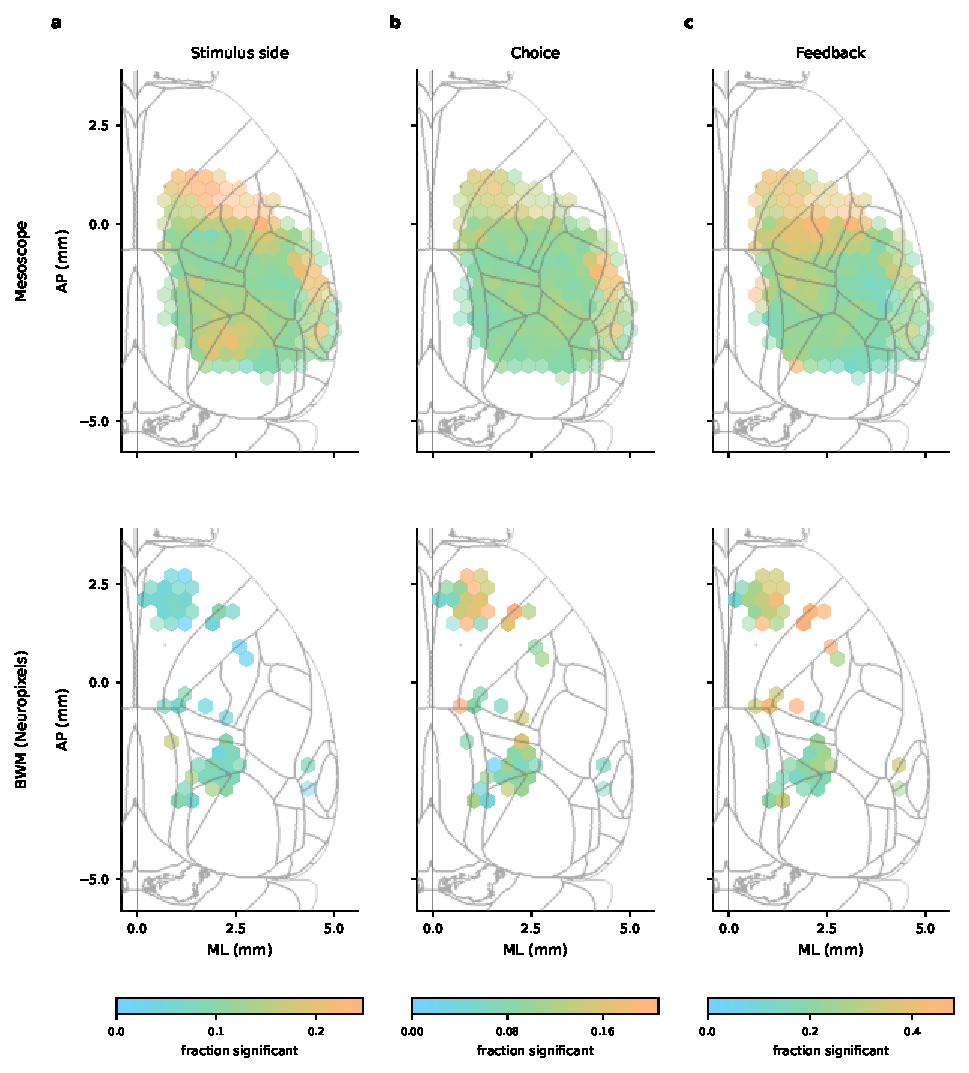
\includegraphics[width=7.00in,height=0.78\textheight,keepaspectratio]{si/si_strict_tuning_panels.pdf}
  \caption{Strict inclusion: only bins (0.4\,mm vertex to vertex, hemispheres folded) with $\geq$3 sessions from $\geq$2 animals, each session contributing $\geq$10 neurons. Isoluminant colour map; opacity encodes the number of animals (2: 50\,\%, 3: 75\,\%, $\geq$4: 100\,\%), so bins backed by few animals fade towards white. Mesoscope top row, BWM bottom row. \textbf{a} Fraction of testable neurons tuned to stimulus side ($p<0.05$), pooled over the included sessions. \textbf{b} Same for choice. \textbf{c} Same for feedback.}
  \label{fig:si_strict_tuning}
\end{figure}
